% answers.tex —— 2016 年·北京卷·理科 · 参考答案与详细解析片段
% 由 tools/generate_projects.py 依来源总账自 2016/2016_数学真题_北京理_试题.md + 2016/2016_数学真题_北京理_解析正文.md + 2016/2016_数学真题_北京理_答案要点.md 生成，勿手改（改源 MD 后重跑）


\begin{gktip}
固定原卷不附官方答案。以下为独立推导并经异人盲核对照的解析（非官方答案，等级 D）。第 6 题的三视图还原以原 PDF 投影关系为准。
\end{gktip}

\begin{answer}
\gksolhead{1}{}

\textbf{题目}：

已知集合 \(A=\{x\mid |x|<2\}\)，\(B=\{-1,0,1,2,3\}\)，则 \(A\cap B=\)（　）

（A）\(\{0,1\}\)　（B）\(\{0,1,2\}\)　（C）\(\{-1,0,1\}\)　（D）\(\{-1,0,1,2\}\)

\Needspace{4\baselineskip}
\textbf{解析}

由 \(|x|<2\) 得 \(-2<x<2\)，故 \(A=(-2,2)\)；与 \(B=\{-1,0,1,2,3\}\) 求交，只有 \(-1,0,1\) 同时属于两者。

\gkanswer{答案：C，\(\{-1,0,1\}\)}

\end{answer}
\begin{answer}
\gksolhead{2}{}

\textbf{题目}：

\Needspace{5\baselineskip}
若 \(x,y\) 满足
\nopagebreak[4]
\[
\begin{cases}
2x-y\leqslant 0,\\
x+y\leqslant 3,\\
x\geqslant 0,
\end{cases}
\]
则 \(2x+y\) 的最大值为（　）

（A）\(0\)　（B）\(3\)　（C）\(4\)　（D）\(5\)

\Needspace{4\baselineskip}
\textbf{解析}

可行域由 \(2x-y\leqslant0\)、\(x+y\leqslant3\)、\(x\geqslant0\) 围成，其顶点为 \((0,0)\)、\((0,3)\) 与直线 \(2x-y=0\)、\(x+y=3\) 的交点 \((1,2)\)。目标函数 \(z=2x+y\) 在这三个顶点处分别取值 \(0,3,4\)，故最大值为 \(4\)。

\gkanswer{答案：C，\(4\)}

\end{answer}
\begin{answer}
\gksolhead{3}{}

\textbf{题目}：

执行如图所示的程序框图，若输入的 \(a\) 值为 \(1\)，则输出的 \(k\) 值为（　）
\nopagebreak[4]
\begin{center}% 第 3 题程序框图：按固定源 PDF 的框图结构逐一重绘（框形、分支标签与回边走向照原图）。
\begin{tikzpicture}[node distance=4mm,>=stealth,every node/.style={font=\small},
  term/.style={draw,rounded corners,minimum width=1.6cm,minimum height=6mm},
  box/.style={draw,minimum width=2.9cm,minimum height=6mm},
  io/.style={draw,trapezium,trapezium left angle=70,trapezium right angle=110,minimum width=2.9cm,minimum height=6mm},
  decision/.style={draw,diamond,aspect=2.2,inner sep=1pt}]
\node[term] (start) {开始};
\node[io,below=of start] (input) {输入 \(a\)};
\node[box,below=of input] (init) {\(k=0,\ b=a\)};
\node[box,below=of init] (assign) {\(a=\dfrac{-1}{1+a}\)};
\node[decision,below=of assign] (test) {\(a=b\)};
\node[io,below=of test] (out) {输出 \(k\)};
\node[term,below=of out] (end) {结束};
\node[box,right=10mm of test] (inc) {\(k=k+1\)};
\draw[->] (start)--(input) (input)--(init) (init)--(assign) (assign)--(test);
\draw[->] (test.south)--node[right]{是}(out.north);
\draw[->] (out)--(end);
\draw[->] (test.east)--node[above]{否}(inc.west);
\draw[->] (inc.north)--++(0,10mm) -| (assign.north);
\end{tikzpicture}
\end{center}
\nopagebreak[4]
（A）\(1\)　（B）\(2\)　（C）\(3\)　（D）\(4\)

\Needspace{4\baselineskip}
\textbf{解析}

初值 \(a=1\)，\(b=a=1\)，\(k=0\)。第一次：\(a=\dfrac{-1}{1+1}=-\dfrac12\neq b\)，\(k=1\)；第二次：\(a=\dfrac{-1}{1-\frac12}=-2\neq b\)，\(k=2\)；第三次：\(a=\dfrac{-1}{1-2}=1=b\)，循环结束，输出 \(k=2\)。

\gkanswer{答案：B，\(2\)}

\end{answer}
\begin{answer}
\gksolhead{4}{}

\textbf{题目}：

设 \(\boldsymbol{a},\boldsymbol{b}\) 是向量，则“\(|\boldsymbol{a}|=|\boldsymbol{b}|\)”是“\(|\boldsymbol{a}+\boldsymbol{b}|=|\boldsymbol{a}-\boldsymbol{b}|\)”的（　）

（A）充分而不必要条件　（B）必要而不充分条件　（C）充分必要条件　（D）既不充分也不必要条件

\Needspace{4\baselineskip}
\textbf{解析}

\(|\boldsymbol a+\boldsymbol b|^2-|\boldsymbol a-\boldsymbol b|^2=4\boldsymbol a\cdot\boldsymbol b\)，故 \(|\boldsymbol a+\boldsymbol b|=|\boldsymbol a-\boldsymbol b|\) 等价于 \(\boldsymbol a\cdot\boldsymbol b=0\)（两向量垂直），而 \(|\boldsymbol a|=|\boldsymbol b|\) 与垂直性互不蕴含：取 \(\boldsymbol a=\boldsymbol b\neq\boldsymbol 0\) 知前者成立而后者不成立，取 \(\boldsymbol a=(1,0),\boldsymbol b=(0,2)\) 知后者成立而前者不成立。故为既不充分也不必要条件。

\gkanswer{答案：D，既不充分也不必要条件}

\end{answer}
\begin{answer}
\gksolhead{5}{}

\textbf{题目}：

已知 \(x,y\in\mathbf{R}\)，且 \(x>y>0\)，则（　）

（A）\(\dfrac{1}{x}-\dfrac{1}{y}>0\)　（B）\(\sin x-\sin y>0\)　（C）\(\left(\dfrac{1}{2}\right)^{x}-\left(\dfrac{1}{2}\right)^{y}<0\)　（D）\(\ln x+\ln y>0\)

\Needspace{4\baselineskip}
\textbf{解析}

由 \(x>y>0\) 及 \(y=\left(\dfrac12\right)^x\) 单调递减，得 \(\left(\dfrac12\right)^x<\left(\dfrac12\right)^y\)，故（C）成立。其余各项均有反例：取 \(x=1,y=\dfrac12\) 可否定（A）；取 \(x=2\pi,y=\dfrac{\pi}{2}\) 可否定（B）；取 \(x=y=\dfrac12\)（极限情形）或以 \(x=1.1,y=1\) 知 \(\ln x+\ln y=\ln(xy)\) 可小于 \(0\)，否定（D）。

\gkanswer{答案：C，\(\left(\dfrac12\right)^{x}-\left(\dfrac12\right)^{y}<0\)}

\end{answer}
\begin{answer}
\gksolhead{6}{}

\textbf{题目}：

某三棱锥的三视图如图所示，则该三棱锥的体积为（　）
\nopagebreak[4]
\begin{center}% 第 6 题三视图：按固定源 PDF 的投影轮廓与尺寸线位置重绘（尺寸数字只保留原图印出的 1、1、1、1）。
\begin{tikzpicture}[every node/.style={font=\small},scale=0.9,line cap=round,line join=round]
% 正（主）视图：尖顶在左上，底边在右下，无尺寸标注
\draw (0,1.0)--(0.98,0)--(1.98,0)--cycle;
\node[below] at (0.99,-0.28) {正（主）视图};
% 侧（左）视图：直角在左下；左侧竖直尺寸线 1，下方水平尺寸线 1
\draw (2.9,0)--(2.9,1.0)--(3.88,0)--cycle;
\draw[<->] (2.72,0)--(2.72,1.0); \node[left] at (2.72,0.5) {1};
\draw[<->] (2.9,-0.20)--(3.88,-0.20); \node[below] at (3.39,-0.20) {1};
\node[below] at (3.39,-0.62) {侧（左）视图};
% 俯视图：直角在右上；上边长 2（两段各 1），上边中点到右下顶点为虚线
\draw (0,-1.98)--(1.98,-1.98)--(1.98,-2.96)--cycle;
\draw[dashed] (0.99,-1.98)--(1.98,-2.96);
\draw[<->] (0,-1.76)--(0.99,-1.76); \node[above] at (0.495,-1.76) {1};
\draw[<->] (0.99,-1.76)--(1.98,-1.76); \node[above] at (1.485,-1.76) {1};
\node[below] at (0.99,-3.30) {俯视图};
\end{tikzpicture}
\end{center}
\nopagebreak[4]
（A）\(\dfrac{1}{6}\)　（B）\(\dfrac{1}{3}\)　（C）\(\dfrac{1}{2}\)　（D）\(1\)

\Needspace{4\baselineskip}
\textbf{解析}

\Needspace{5\baselineskip}
由三视图还原该三棱锥：侧（左）视图是两直角边均为 \(1\) 的直角三角形，故几何体的高为 \(1\)；正（主）视图说明顶点（最高点）位于左端（\(x=0\)）的正上方；俯视图的轮廓是上边长 \(2\)（两段各 \(1\)）、右边长 \(1\) 的直角三角形，其中由上边中点连到右下顶点的虚线是俯视时被侧面遮住的底面棱。于是底面为俯视图中以 \((1,0),(2,0),(2,1)\) 为顶点的直角三角形，两直角边长均为 \(1\)，面积 \(S=\dfrac12\)，棱锥高 \(h=1\)。

\nopagebreak[4]
\[
V=\frac13Sh=\frac13\times\frac12\times1=\frac16.
\]

\gkanswer{答案：A，\(\dfrac16\)}

\end{answer}
\begin{answer}
\gksolhead{7}{}

\textbf{题目}：

将函数 \(y=\sin\left(2x-\dfrac{\pi}{3}\right)\) 图象上的点 \(P\left(\dfrac{\pi}{4},t\right)\) 向左平移 \(s\)（\(s>0\)）个单位长度得到点 \(P'\)。若 \(P'\) 位于函数 \(y=\sin 2x\) 的图象上，则（　）

（A）\(t=\dfrac{1}{2}\)，\(s\) 的最小值为 \(\dfrac{\pi}{6}\)　（B）\(t=\dfrac{\sqrt{3}}{2}\)，\(s\) 的最小值为 \(\dfrac{\pi}{6}\)

（C）\(t=\dfrac{1}{2}\)，\(s\) 的最小值为 \(\dfrac{\pi}{3}\)　（D）\(t=\dfrac{\sqrt{3}}{2}\)，\(s\) 的最小值为 \(\dfrac{\pi}{3}\)

\Needspace{4\baselineskip}
\textbf{解析}

\Needspace{5\baselineskip}
\(t=\sin\left(2\cdot\dfrac{\pi}{4}-\dfrac{\pi}{3}\right)=\sin\dfrac{\pi}{6}=\dfrac12\)。向左平移 \(s\) 后 \(P'\left(\dfrac{\pi}{4}-s,\ t\right)\)，由 \(P'\) 在 \(y=\sin 2x\) 上得

\nopagebreak[4]
\[
\frac12=\sin\left(2\left(\frac{\pi}{4}-s\right)\right)=\sin\left(\frac{\pi}{2}-2s\right)=\cos 2s,
\]

故 \(2s=2k\pi\pm\dfrac{\pi}{3}\)，取 \(s>0\) 的最小值 \(s=\dfrac{\pi}{6}\)。

\gkanswer{答案：A，\(t=\dfrac12\)，\(s\) 的最小值为 \(\dfrac{\pi}{6}\)}

\end{answer}
\begin{answer}
\gksolhead{8}{}

\textbf{题目}：

袋中装有偶数个球，其中红球、黑球各占一半。甲、乙、丙是三个空盒。每次从袋中任意取出两个球，将其中一个球放入甲盒，如果这个球是红球，就将另一个球放入乙盒，否则就放入丙盒。重复上述过程，直到袋中所有球都被放入盒中，则（　）

（A）乙盒中黑球不多于丙盒中黑球　（B）乙盒中红球与丙盒中黑球一样多

（C）乙盒中红球不多于丙盒中红球　（D）乙盒中黑球与丙盒中红球一样多

\Needspace{4\baselineskip}
\textbf{解析}

设每轮取出的两球中先放入甲盒的球为 \(X\)，另一球为 \(Y\)：\(X\) 为红球时 \(Y\) 入乙盒，\(X\) 为黑球时 \(Y\) 入丙盒。记四类轮数为 \(a(X\) 红 \(Y\) 红\()\)、\(b(X\) 红 \(Y\) 黑\()\)、\(c(X\) 黑 \(Y\) 红\()\)、\(d(X\) 黑 \(Y\) 黑\()\)。红球总数为 \(a+b+a+c=2a+b+c\)，黑球总数为 \(b+d+c+d=b+c+2d\)；红黑各占一半，故 \(2a+b+c=b+c+2d\)，得 \(a=d\)。

乙盒中红球数正是 \(a\)（\(X\) 红且 \(Y\) 红），丙盒中黑球数正是 \(d\)（\(X\) 黑且 \(Y\) 黑），故两者一样多。

\gkanswer{答案：B，乙盒中红球与丙盒中黑球一样多}

\end{answer}
\begin{answer}
\gksolhead{9}{}

\textbf{题目}：

设 \(a\in\mathbf{R}\)，若复数 \((1+\mathrm{i})(a+\mathrm{i})\) 在复平面内对应的点位于实轴上，则 \(a=\underline{\qquad}\)。

\Needspace{4\baselineskip}
\textbf{解析}

\((1+\mathrm i)(a+\mathrm i)=a+\mathrm i+a\mathrm i+\mathrm i^2=(a-1)+(a+1)\mathrm i\)，对应点位于实轴上当且仅当虚部为零，即 \(a+1=0\)。

\gkanswer{答案：\(-1\)}

\end{answer}
\begin{answer}
\gksolhead{10}{}

\textbf{题目}：

在 \((1-2x)^{6}\) 的展开式中，\(x^{2}\) 的系数为 \(\underline{\qquad}\)。（用数字作答）

\Needspace{4\baselineskip}
\textbf{解析}

展开式通项为 \(\mathrm C_6^{k}(-2x)^{k}\)，取 \(k=2\) 得 \(x^2\) 的系数 \(\mathrm C_6^{2}\cdot(-2)^2=15\times4=60\)。

\gkanswer{答案：\(60\)}

\end{answer}
\begin{answer}
\gksolhead{11}{}

\textbf{题目}：

在极坐标系中，直线 \(\rho\cos\theta-\sqrt{3}\rho\sin\theta-1=0\) 与圆 \(\rho=2\cos\theta\) 交于 \(A,B\) 两点，则 \(|AB|=\underline{\qquad}\)。

\Needspace{4\baselineskip}
\textbf{解析}

\Needspace{5\baselineskip}
由 \(x=\rho\cos\theta,\ y=\rho\sin\theta\) 化直角坐标：直线为 \(x-\sqrt3y-1=0\)，圆 \(\rho=2\cos\theta\) 两边乘 \(\rho\) 得 \(\rho^2=2\rho\cos\theta\)，即 \(x^2+y^2=2x\)，圆心 \((1,0)\)、半径 \(1\)。圆心到直线的距离

\nopagebreak[4]
\[
\frac{|1-\sqrt3\cdot0-1|}{\sqrt{1+3}}=0,
\]

即直线过圆心，故弦 \(AB\) 为直径，\(|AB|=2\)。

\gkanswer{答案：\(2\)}

\end{answer}
\begin{answer}
\gksolhead{12}{}

\textbf{题目}：

已知 \(\{a_{n}\}\) 为等差数列，\(S_{n}\) 为其前 \(n\) 项和，若 \(a_{1}=6\)，\(a_{3}+a_{5}=0\)，则 \(S_{6}=\underline{\qquad}\)。

\Needspace{4\baselineskip}
\textbf{解析}

\Needspace{5\baselineskip}
设公差为 \(d\)。由 \(a_3+a_5=(a_1+2d)+(a_1+4d)=2a_1+6d=12+6d=0\) 得 \(d=-2\)，故

\nopagebreak[4]
\[
S_6=6a_1+\frac{6\times5}{2}d=36+15\times(-2)=6.
\]

\gkanswer{答案：\(6\)}

\end{answer}
\begin{answer}
\gksolhead{13}{}

\textbf{题目}：

双曲线 \(\dfrac{x^{2}}{a^{2}}-\dfrac{y^{2}}{b^{2}}=1\)（\(a>0\)，\(b>0\)）的渐近线为正方形 \(OABC\) 的边 \(OA\)，\(OC\) 所在的直线，点 \(B\) 为该双曲线的焦点，若正方形 \(OABC\) 的边长为 \(2\)，则 \(a=\underline{\qquad}\)。

\Needspace{4\baselineskip}
\textbf{解析}

双曲线的渐近线为 \(y=\pm\dfrac ba x\)，题设中它们是正方形相邻两边 \(OA\)、\(OC\) 所在直线，故两渐近线互相垂直，\(\dfrac ba\cdot\left(-\dfrac ba\right)=-1\)，得 \(a=b\)。此时 \(c^2=a^2+b^2=2a^2\)。又 \(B\) 为与 \(O\) 相对的正方形顶点，边长 \(2\) 时 \(|OB|=2\sqrt2\)，即 \(c=2\sqrt2\)，于是 \(2a^2=8\)。

\gkanswer{答案：\(2\)}

\end{answer}
\begin{answer}
\gksolhead{14}{}

\textbf{题目}：

\Needspace{5\baselineskip}
设函数
\nopagebreak[4]
\[
f(x)=\begin{cases}
x^{3}-3x, & x\leqslant a,\\
-2x, & x>a.
\end{cases}
\]
① 若 \(a=0\)，则 \(f(x)\) 的最大值为 \(\underline{\qquad}\)；

② 若 \(f(x)\) 无最大值，则实数 \(a\) 的取值范围是 \(\underline{\qquad}\)。

\Needspace{4\baselineskip}
\textbf{解析}

\gksubpart{①}

\(a=0\) 时 \(f(x)=x^3-3x\ (x\leqslant0)\)，在 \(x=-1\) 处取极大值 \(f(-1)=-1+3=2\)，且 \(x\to-\infty\) 时 \(f(x)\to-\infty\)，\(f(0)=0<2\)，故最大值为 \(2\)。

\gksubpart{②}

\(f\) 在 \(x\leqslant a\) 上的最大值在驻点 \(x=-1\)（若 \(-1\leqslant a\)）或端点 \(x=a\) 处取得。当 \(a\geqslant-1\) 时，\(x=-1\) 属于该段，最大值 \(f(-1)=2\) 被取到；当 \(a<-1\) 时，\(x^3-3x\) 在 \((-\infty,a]\) 上单调递增，该段最大值为 \(f(a)=a^3-3a\)（取得到），而 \(x>a\) 段为 \(-2x<-2a\)，其上确界 \(-2a\) 取不到；由 \(a<-1\) 得 \(-2a>a^3-3a\)，故整体无最大值。所以 \(f(x)\) 无最大值的充要条件是 \(a<-1\)。

\gkanswer{答案：① \(2\)；② \((-\infty,-1)\)。}

\end{answer}
\begin{answer}
\gksolhead{15}{}

\textbf{题目}：

在 \(\triangle ABC\) 中，\(a^{2}+c^{2}=b^{2}+\sqrt{2}ac\)。

（1） 求 \(\angle B\) 的大小；

（2） 求 \(\sqrt{2}\cos A+\cos C\) 的最大值。

\Needspace{4\baselineskip}
\textbf{解析}

\gksubpart{(1)}

\Needspace{5\baselineskip}
由余弦定理

\nopagebreak[4]
\[
\cos B=\frac{a^2+c^2-b^2}{2ac}=\frac{\sqrt2ac}{2ac}=\frac{\sqrt2}{2},
\]

又 \(B\in(0,\pi)\)，故 \(B=\dfrac{\pi}{4}\)。

\gksubpart{(2)}

\Needspace{5\baselineskip}
\(A+C=\pi-B=\dfrac{3\pi}{4}\)，故

\nopagebreak[4]
\[
\begin{aligned}
\sqrt2\cos A+\cos C&=\sqrt2\cos A+\cos\left(\frac{3\pi}{4}-A\right)\\
&=\sqrt2\cos A-\frac{\sqrt2}{2}\cos A+\frac{\sqrt2}{2}\sin A\\
&=\frac{\sqrt2}{2}(\cos A+\sin A)=\sin\left(A+\frac{\pi}{4}\right).
\end{aligned}
\]

由 \(A\in\left(0,\dfrac{3\pi}{4}\right)\) 得 \(A+\dfrac{\pi}{4}\in\left(\dfrac{\pi}{4},\pi\right)\)，当 \(A+\dfrac{\pi}{4}=\dfrac{\pi}{2}\) 即 \(A=B=\dfrac{\pi}{4}\) 时取最大值 \(1\)（此时 \(C=\dfrac{\pi}{2}\)，三角形存在）。

\gkanswer{答案（1）：\(B=\dfrac{\pi}{4}\)。}

\gkanswer{答案（2）：最大值为 \(1\)。}

\end{answer}
\begin{answer}
\gksolhead{16}{}

\textbf{题目}：

\(A,B,C\) 三个班共有 \(100\) 名学生，为调查他们的体育锻炼情况，通过分层抽样获得了部分学生一周的锻炼时间，数据如表（单位：小时）：

\begin{center}
\begin{tabular}{ll}
\toprule
班级 & 锻炼时间 \\
\midrule
\(A\) 班 & 6　6.5　7　7.5　8 \\
\(B\) 班 & 6　7　8　9　10　11　12 \\
\(C\) 班 & 3　4.5　6　7.5　9　10.5　12　13.5 \\
\bottomrule
\end{tabular}
\end{center}

（1） 试估计 \(C\) 班的学生人数；

（2） 从 \(A\) 班和 \(C\) 班抽出的学生中，各随机选取一个人，\(A\) 班选出的人记为甲，\(C\) 班选出的人记为乙。假设所有学生的锻炼时间相对独立，求该周甲的锻炼时间比乙的锻炼时间长的概率；

（3） 再从 \(A,B,C\) 三班中各随机抽取一名学生，他们该周锻炼时间分别是 \(7,9,8.25\)（单位：小时），这 \(3\) 个新数据与表格中的数据构成的新样本的平均数记为 \(\mu_{1}\)，表格中数据的平均数记为 \(\mu_{0}\)，试判断 \(\mu_{0}\) 和 \(\mu_{1}\) 的大小。（结论不要求证明）

\Needspace{4\baselineskip}
\textbf{解析}

\gksubpart{(1)}

样本共 \(5+7+8=20\) 人，其中 \(C\) 班 \(8\) 人，占比 \(\dfrac{8}{20}=\dfrac25\)。按分层抽样比例估计，\(C\) 班学生人数约为 \(100\times\dfrac25=40\)。

\gksubpart{(2)}

甲、乙的锻炼时间相互独立，各 \(5\times8=40\) 种等可能组合。逐一计数甲大于乙的组合数：甲取 \(6\) 时 \(2\) 种，取 \(6.5\) 时 \(3\) 种（\(3,4.5,6\)），取 \(7\) 时 \(3\) 种，取 \(7.5\) 时 \(3\) 种，取 \(8\) 时 \(4\) 种，合计 \(15\) 种。故所求概率为 \(\dfrac{15}{40}=\dfrac38\)。

\gksubpart{(3)}

\Needspace{5\baselineskip}
表格中 \(20\) 个数据的和为 \(35+63+66=164\)，\(\mu_0=\dfrac{164}{20}=8.2\)。加入 \(7,9,8.25\) 后

\nopagebreak[4]
\[
\mu_1=\frac{164+24.25}{23}=\frac{188.25}{23}\approx8.1848<8.2,
\]

故 \(\mu_0>\mu_1\)。

\gkanswer{答案（1）：\(40\) 人。}

\gkanswer{答案（2）：\(\dfrac38\)。}

\gkanswer{答案（3）：\(\mu_0>\mu_1\)。}

\end{answer}
\begin{answer}
\gksolhead{17}{}

\textbf{题目}：

如图，在四棱锥 \(P-ABCD\) 中，平面 \(PAD\perp\) 平面 \(ABCD\)，\(PA\perp PD\)，\(PA=PD\)，\(AB\perp AD\)，\(AB=1\)，\(AD=2\)，\(AC=CD=\sqrt{5}\)。
\nopagebreak[4]
\begin{center}% 第 17 题四棱锥 P-ABCD：按固定源 PDF 的顶点相对位置重绘；虚线仅 DA、AC 两条。
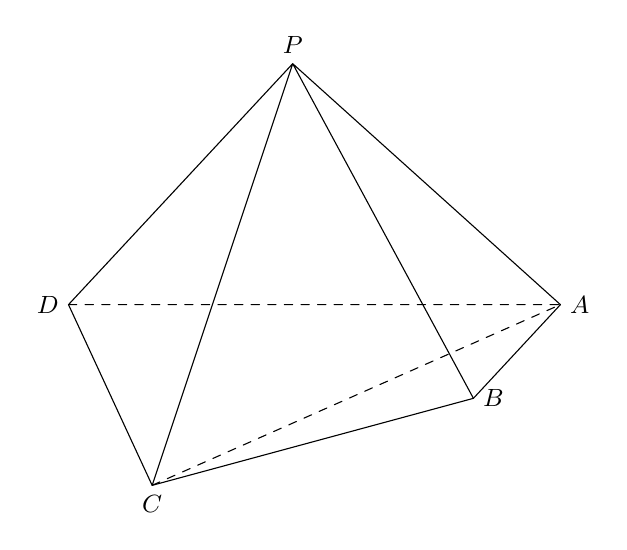
\begin{tikzpicture}[line cap=round,line join=round,font=\small,scale=0.85]
\coordinate (P) at (2.1,6.3);
\coordinate (D) at (-1.25,2.7);
\coordinate (A) at (6.1,2.7);
\coordinate (B) at (4.8,1.3);
\coordinate (C) at (0,0);
\draw (P)--(D) (P)--(A) (P)--(B) (P)--(C);
\draw (D)--(C) (C)--(B) (B)--(A);
\draw[dashed] (D)--(A) (C)--(A);
\node[above] at (P) {$P$};
\node[left] at (D) {$D$};
\node[right] at (A) {$A$};
\node[right] at (B) {$B$};
\node[below] at (C) {$C$};
\end{tikzpicture}
\end{center}
\nopagebreak[4]
（1） 求证：\(PD\perp\) 平面 \(PAB\)；

（2） 求直线 \(PB\) 与平面 \(PCD\) 所成角的正弦值；

（3） 在棱 \(PA\) 上是否存在点 \(M\)，使得 \(BM\parallel\) 平面 \(PCD\)？若存在，求 \(\dfrac{AM}{AP}\) 的值；若不存在，说明理由。

\Needspace{4\baselineskip}
\textbf{解析}

\gksubpart{(1)}

平面 \(PAD\perp\) 平面 \(ABCD\)，交线为 \(AD\)；又 \(AB\perp AD\)，\(AB\subset\) 平面 \(ABCD\)，故 \(AB\perp\) 平面 \(PAD\)。于是 \(AB\perp PD\)。又已知 \(PA\perp PD\)，\(PA\) 与 \(AB\) 是平面 \(PAB\) 内两条相交直线，故 \(PD\perp\) 平面 \(PAB\)。

\gksubpart{(2)}

取 \(AD\) 中点 \(O\)。由 \(PA=PD=\dfrac{\sqrt2}{2}AD=\sqrt2\) 且 \(PA\perp PD\) 得 \(PO\perp AD\) 且 \(PO=\dfrac{AD}{2}=1\)；又平面 \(PAD\perp\) 平面 \(ABCD\)，故 \(PO\perp\) 平面 \(ABCD\)。

以 \(O\) 为原点，\(OD\) 方向为 \(x\) 轴正方向，建立空间直角坐标系，则 \(A(-1,0,0)\)，\(D(1,0,0)\)，\(P(0,0,1)\)。由 \(AB\perp AD\)、\(AB=1\) 得 \(B(-1,1,0)\)（取其一侧即可，另一侧镜像不影响结论）；由 \(AC=CD=\sqrt5\) 且 \(C\) 在 \(AD\) 的垂直平分面上，得 \(C(0,2,0)\)。

\Needspace{5\baselineskip}
\(\overrightarrow{PB}=(-1,1,-1)\)。平面 \(PCD\) 中 \(\overrightarrow{PC}=(0,2,-1)\)、\(\overrightarrow{PD}=(1,0,-1)\)，取法向量

\nopagebreak[4]
\[
\boldsymbol n=\overrightarrow{PC}\times\overrightarrow{PD}=(-2,-1,-2),\qquad|\boldsymbol n|=3 .
\]

\Needspace{5\baselineskip}
设 \(PB\) 与平面 \(PCD\) 所成角为 \(\theta\)，则

\nopagebreak[4]
\[
\sin\theta=\frac{|\overrightarrow{PB}\cdot\boldsymbol n|}{|\overrightarrow{PB}|\,|\boldsymbol n|}
=\frac{|2-1+2|}{\sqrt3\times3}=\frac{\sqrt3}{3}.
\]

\gksubpart{(3)}

\Needspace{5\baselineskip}
设 \(M=A+\lambda(P-A)=(-1+\lambda,0,\lambda)\)，\(\lambda\in[0,1]\)，则 \(\dfrac{AM}{AP}=\lambda\)，且 \(\overrightarrow{BM}=(\lambda,-1,\lambda)\)。\(BM\parallel\) 平面 \(PCD\) 当且仅当 \(\overrightarrow{BM}\perp\boldsymbol n\)：

\nopagebreak[4]
\[
-2\lambda+1-2\lambda=0\ \Longrightarrow\ \lambda=\frac14 .
\]

故存在这样的点 \(M\)，此时 \(\dfrac{AM}{AP}=\dfrac14\)。

\gkanswer{答案（1）：见解析版}

\gkanswer{答案（2）：\(\dfrac{\sqrt3}{3}\)。}

\gkanswer{答案（3）：存在，\(\dfrac{AM}{AP}=\dfrac14\)。}

\end{answer}
\begin{answer}
\gksolhead{18}{}

\textbf{题目}：

设函数 \(f(x)=x\mathrm{e}^{a-x}+bx\)，曲线 \(y=f(x)\) 在点 \((2,f(2))\) 处的切线方程为 \(y=(\mathrm{e}-1)x+4\)。

（1） 求 \(a,b\) 的值；

（2） 求 \(f(x)\) 的单调区间。

\Needspace{4\baselineskip}
\textbf{解析}

\gksubpart{(1)}

\Needspace{5\baselineskip}
\(f'(x)=\mathrm e^{a-x}(1-x)+b\)。由切线方程得 \(f(2)=2(\mathrm e-1)+4=2\mathrm e+2\)，\(f'(2)=\mathrm e-1\)。记 \(u=\mathrm e^{a-2}\)，则

\nopagebreak[4]
\[
\begin{cases}
2u+2b=2\mathrm e+2,\\
-u+b=\mathrm e-1,
\end{cases}
\]

第二式乘 \(2\) 与第一式相加得 \(4b=4\mathrm e\)，故 \(b=\mathrm e\)；回代得 \(u=1\)，即 \(\mathrm e^{a-2}=1\)，\(a=2\)。

\gksubpart{(2)}

\Needspace{5\baselineskip}
此时 \(f(x)=x\mathrm e^{2-x}+\mathrm e x\)，且

\nopagebreak[4]
\[
f'(x)=\mathrm e^{2-x}(1-x)+\mathrm e .
\]

记 \(g(x)=\mathrm e^{2-x}(1-x)\)，则 \(g'(x)=\mathrm e^{2-x}(x-2)\)：\(g\) 在 \((-\infty,2)\) 上递减、在 \((2,+\infty)\) 上递增，故 \(g(x)\geqslant g(2)=0\) 对一切 \(x\) 成立。于是 \(f'(x)\geqslant\mathrm e>0\)。

所以 \(f(x)\) 在 \((-\infty,+\infty)\) 上单调递增，无单调递减区间。

\gkanswer{答案（1）：\(a=2\)，\(b=\mathrm e\)。}

\gkanswer{答案（2）：单调递增区间为 \((-\infty,+\infty)\)，无递减区间。}

\end{answer}
\begin{answer}
\gksolhead{19}{}

\textbf{题目}：

已知椭圆 \(C:\dfrac{x^{2}}{a^{2}}+\dfrac{y^{2}}{b^{2}}=1\)（\(a>b>0\)）的离心率为 \(\dfrac{\sqrt{3}}{2}\)，\(A(a,0)\)，\(B(0,b)\)，\(O(0,0)\)，\(\triangle OAB\) 的面积为 \(1\)。

（1） 求椭圆 \(C\) 的方程；

（2） 设 \(P\) 是椭圆 \(C\) 上一点，直线 \(PA\) 与 \(y\) 轴交于点 \(M\)，直线 \(PB\) 与 \(x\) 轴交于点 \(N\)。求证：\(|AN|\cdot|BM|\) 为定值。

\Needspace{4\baselineskip}
\textbf{解析}

\gksubpart{(1)}

由离心率 \(\dfrac ca=\dfrac{\sqrt3}{2}\) 得 \(b^2=a^2-c^2=a^2-\dfrac34a^2=\dfrac{a^2}{4}\)，即 \(b=\dfrac a2\)。又 \(\triangle OAB\) 的面积为 \(1\)，即 \(\dfrac12ab=1\)，代入得 \(\dfrac12\cdot a\cdot\dfrac a2=1\)，\(a^2=4\)。故 \(a=2\)，\(b=1\)。

\gksubpart{(2)}

设 \(P(x_0,y_0)\) 为椭圆上一点（\(P\neq A,B\)），\(\dfrac{x_0^2}{4}+y_0^2=1\)。

\Needspace{5\baselineskip}
直线 \(PA\) 过 \(A(2,0)\)，斜率 \(\dfrac{y_0}{x_0-2}\)，与 \(y\) 轴交于

\nopagebreak[4]
\[
M\left(0,\ -\frac{2y_0}{x_0-2}\right),\qquad
|BM|=\left|1+\frac{2y_0}{x_0-2}\right|=\frac{|x_0-2+2y_0|}{|x_0-2|}.
\]

\Needspace{5\baselineskip}
直线 \(PB\) 过 \(B(0,1)\)，斜率 \(\dfrac{y_0-1}{x_0}\)，与 \(x\) 轴交于

\nopagebreak[4]
\[
N\left(-\frac{x_0}{y_0-1},\ 0\right),\qquad
|AN|=\left|2+\frac{x_0}{y_0-1}\right|=\frac{|x_0+2y_0-2|}{|y_0-1|}.
\]

\Needspace{5\baselineskip}
两式相乘并利用 \(x_0^2+4y_0^2=4\)：

\nopagebreak[4]
\[
|AN|\cdot|BM|=\frac{|x_0+2y_0-2|\,|x_0-2+2y_0|}{|x_0-2|\,|y_0-1|}
=\frac{(x_0+2y_0-2)^2}{|(x_0-2)(y_0-1)|}.
\]

\Needspace{5\baselineskip}
由 \(\dfrac{x_0^2}{4}+y_0^2=1\) 得 \(x_0^2=4-4y_0^2\)，代入展开：

\nopagebreak[4]
\[
(x_0+2y_0-2)^2=x_0^2+4y_0^2+4+4x_0y_0-4x_0-8y_0=4(2+x_0y_0-x_0-2y_0),
\]

\Needspace{5\baselineskip}
而

\nopagebreak[4]
\[
(x_0-2)(y_0-1)=x_0y_0-x_0-2y_0+2,
\]

\Needspace{5\baselineskip}
两者括号内完全相同，故

\nopagebreak[4]
\[
|AN|\cdot|BM|=\left|\frac{(x_0+2y_0-2)^2}{(x_0-2)(y_0-1)}\right|=4
\]

为定值。

\gkanswer{答案（1）：\(\dfrac{x^2}{4}+y^2=1\)。}

\gkanswer{答案（2）：见解析版}

\end{answer}
\begin{answer}
\gksolhead{20}{}

\textbf{题目}：

设数列 \(A:a_{1},a_{2},\cdots,a_{N}\)（\(N\geqslant 2\)）。如果对小于 \(n\)（\(2\leqslant n\leqslant N\)）的每个正整数 \(k\) 都有 \(a_{k}<a_{n}\)，则称 \(n\) 是数列 \(A\) 的一个“\(G\) 时刻”。记 \(G(A)\) 是数列 \(A\) 的所有“\(G\) 时刻”组成的集合。

（1） 对数列 \(A:-2,2,-1,1,3\)，写出 \(G(A)\) 的所有元素；

（2） 证明：若数列 \(A\) 中存在 \(a_{n}\) 使得 \(a_{n}>a_{1}\)，则 \(G(A)\neq\varnothing\)；

（3） 证明：若数列 \(A\) 满足 \(a_{n}-a_{n-1}\leqslant 1\)（\(n=2,3,\cdots,N\)），则 \(G(A)\) 的元素个数不小于 \(a_{N}-a_{1}\)。

\Needspace{4\baselineskip}
\textbf{解析}

“\(G\) 时刻”即严格前缀最大值的位置：\(n\in G(A)\) 当且仅当 \(a_n>a_k\) 对一切 \(k<n\) 成立，即 \(a_n>M_{n-1}\)，其中 \(M_{n-1}=\max\{a_1,\dots,a_{n-1}\}\)。

\gksubpart{(1)}

\(A:-2,2,-1,1,3\)。\(n=2\)：\(a_2=2>-2\)，是；\(n=3\)：\(a_3=-1<2\)，不是；\(n=4\)：\(a_4=1<2\)，不是；\(n=5\)：\(a_5=3>\max\{-2,2,-1,1\}=2\)，是。故 \(G(A)=\{2,5\}\)。

\gksubpart{(2)}

设 \(a_m=\max\{a_1,a_2,\dots,a_N\}\) 且取 \(m\) 为最大值\textbf{首次}出现的下标。则对一切 \(k<m\) 有 \(a_k<a_m\)，即 \(m\in G(A)\)。题设存在 \(a_n>a_1\)，故最大值 \(a_m\geqslant a_n>a_1\)，从而 \(m\geqslant2\)，\(G(A)\neq\varnothing\)。

\gksubpart{(3)}

设 \(G(A)=\{n_1<n_2<\cdots<n_t\}\)，记 \(b_i=a_{n_i}\)（\(i=1,\dots,t\)）为序列的各级新纪录，\(b_0=a_1\)。

\Needspace{5\baselineskip}
首先证明 \(b_i-b_{i-1}\leqslant1\)（\(i=1,\dots,t\)）：由 \(n_i\) 的定义，对一切 \(k<n_i\) 有 \(a_k<a_{n_i}\)，特别地 \(a_{n_i-1}<a_{n_i}\) 且下标 \(n_i-1\) 不是 \(G\) 时刻（因为 \(n_i\) 是最小的大于 \(n_{i-1}\) 的新纪录位置），故 \(a_{n_i-1}\leqslant b_{i-1}\)；结合题设 \(a_{n_i}-a_{n_i-1}\leqslant1\) 得

\nopagebreak[4]
\[
b_i=a_{n_i}\leqslant a_{n_i-1}+1\leqslant b_{i-1}+1 .
\]

（\(i=1\) 时 \(a_{n_1-1}\leqslant a_1=b_0\)，同法成立。）

\Needspace{5\baselineskip}
又 \(b_t=\max\{a_1,\dots,a_N\}\)，故 \(a_N\leqslant b_t\)。于是

\nopagebreak[4]
\[
a_N-a_1\leqslant b_t-b_0=\sum_{i=1}^{t}(b_i-b_{i-1})\leqslant t=|G(A)|,
\]

即 \(G(A)\) 的元素个数不小于 \(a_N-a_1\)。

\gkanswer{答案（1）：\(G(A)=\{2,5\}\)。}

\gkanswer{答案（2）：见解析版}

\gkanswer{答案（3）：见解析版}

\end{answer}